\chapter{GL-117 Basics}
\label{chap:basics}

Having understood the physical aspects of piloting,
you may now get an introduction to the game itself.

\section{Cockpit controls}
\label{sec:cockpit}

\begin{figure}
\begin{center}
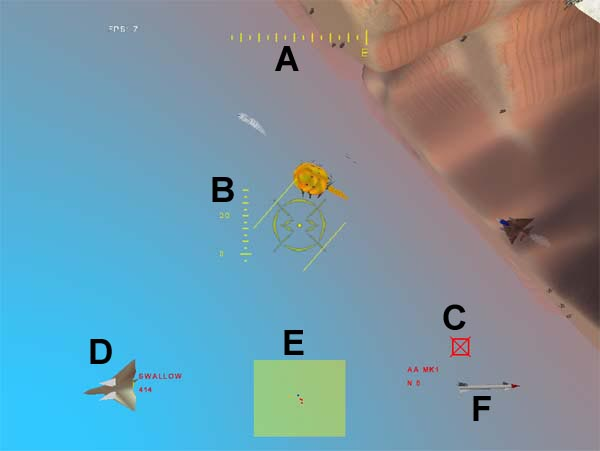
\includegraphics[width=12cm]{hud.jpg}
\caption{A typical HUD of GL-117}
\label{fig:hud}
\end{center}
\end{figure}

Figure \ref{fig:hud} shows a typical \texttt{HUD} (heads up display):
\begin{itemize}
\item{A: your current heading, showing the letters \texttt{'N', 'E', 'S', W'}
to represent north, east, south, west.}
\item{B: your current elevation in degree; the rotating lines reveal the
horizon and thus your roll angle.}
\item{C: the autotargeter shows you the best way to the current target.}
\item{D: your current target}
\item{E: the radar reveals the position of other targets. Enemies are marked red,
allies blue, and the current target is respresented as yellow point.
The screen is only 2D, so it will only reveal the necessary heading to get
other targets.}
\item{F: your currently selected weapon}
\end{itemize}



\section{Input devices}
\label{sec:input_devices}

\emph{GL-117} supports a number of devices depending on \texttt{GLUT} and \texttt{SDL}.
You may choose your preferred input device within the options menu.
It is strongly recommended to use a joystick, however the mouse interface
is also very easy to handle.

\subsection{The keyboard}
\label{subsec:keyboard}

\begin{center}
\begin{tabular}{|c|c|l|l|l|}
\hline
\textsc{Key} & \textsc{Meaning}\\\hline
UP, DOWN & Elevator\\
LEFT, RIGHT & Roll\\
PAGEUP, PAGEDOWN & Rudder\\
1, 2, 3, 4, 5, 6, 7, 8, 9 & Throttle\\
\hline
SPACE & Fire cannon\\
m & Change weapon/missile\\
ENTER & Fire weapon/missile\\
\hline
t & Target next object\\
e & Target nearest enemy\\
\hline
ESC & Main menu\\
\hline
F1 & Cockpit camera\\
F2 & Chase camera\\
F3 & Rear camera\\
F4, F5 & Side cameras\\
F6, F7, F8 & Top cameras\\
\hline
\end{tabular}
\end{center}

\subsection{The mouse}
\label{subsec:mouse}

Moving the mouse up or down will change the elevator to fly a loop, whereas
moving left or right will result in a roll, a slight movement will
affect the rudder.\\
To change your heading, you will thus have to move the mouse cursor completely
to the left/right for a short moment (just figure it out) in order to fly a
quarter roll. Return the mouse cursor to the center immediately!
Then alter the elevator moving the mouse to the top center of your screen to
fly a "loop" parallel to the surface.\\
The left mouse button can be used to fire the cannon, the right button will
fire the weapon/missile, although it is recommended to use the keyboard for
targeting and firing purpose.\\
Look at the keyboard table for a list of keys.\\
Along with the "mouse easy" interface comes the possibility to revert the
elevator controls, called "mouse reverse". Only experienced players should
use this option.

\subsection{The joystick}
\label{subsec:joystick}

The easiest interface to play \emph{GL-117} is likely the joystick.\\
\emph{GL-117} supports up to four joystick axis:
moving the joystick up or down will change the elevator, moving left or right
will affect the aileron, turning the joystick along the rudder will alter
the fighter's rudder settings, and moving the throttle will change
the fighter's throttle.\\\\
Depending on your joystick, \emph{GL-117} supports four buttons:
fire cannon, target nearest enemy, change weapon/missile, fire weapon/missile.\\\\
Any properly installed joystick will be available automatically.


\section{The menu}
\label{sec:menu}

As the menu is almost completely self-explanatory, there is only a brief
description of the different menu items:
\begin{itemize}
\item{The \texttt{PILOTS} menu lets you create and delete pilots. You can
play only one pilot at a time.}
\item{The \texttt{MISSIONS} menu shows all available missions. You have to
succeed in a mission to enable the next one.}
\item{Several \texttt{OPTIONS} may be adjusted: quality, view, sound, music,
difficulty.}
\end{itemize}


\section{Graphics optimization}
\label{sec:graphics_optimization}

To get the best graphics possible on your system, always look at the
\texttt{FPS} rate which describes the number of frames per second.
This rate is directly influenced by the quality and view settings and
should not drop below 20. If your rate is \texttt{perfect}, you should
use higher/better quality and view settings.
You should also try out higher screen resolutions modifying the file
\texttt{conf}. On \texttt{MSWindows} you will find it in the \texttt{saves}
directory, on \texttt{UNIX/Linux} it is stored in the directory
\texttt{\$HOME/.gl-117}.


\section{Score}
\label{sec:score}

Every mission you succeed will earn you a certain score, being calculated
depending on the time it took, the shield you lost, how many targets you
eliminated, and a difficulty bonus.\\
High scores are necessary to get a promotion to a higher military rank.
The difficulty bonus is added to the overall score automatically.
